\documentclass[dvipsnames,border=3pt]{standalone}
\usepackage{tikz}
\usetikzlibrary{arrows}
\usetikzlibrary{shapes}
\usepackage{enumitem}
\usepackage{bm}
\usepackage{mathdots}
\usepackage{amsmath}
\usetikzlibrary{shadings}
\usetikzlibrary{decorations.pathreplacing}
\usepackage{helvet}
\usetikzlibrary{arrows.meta}
\usepackage{graphicx}
\usepackage{pgfplots}
\usepackage{pgfplotstable}
\usepackage{filecontents}
\usetikzlibrary{plotmarks}
\usetikzlibrary{shapes.misc}
\pgfplotsset{compat=newest}

\renewcommand{\familydefault}{\sfdefault}

\definecolor{mylightgray}{cmyk}{0,0,0,0.1}
\usetikzlibrary{arrows,decorations.pathmorphing,backgrounds,fit,positioning,shapes.symbols,chains}

\begin{document}

\begin{tikzpicture}
    % trim=left botm right top
    
    \node at (4.5,2.4) {\LARGE \textbf{Mixed effects data: interactions and main effects}};
    
    % 1 - 2
    \draw[-latex, line width=1mm,draw=gray!70] (3.62,0) -- (5.23,0);
    
    % 2 - 3
    \draw[-latex, line width=1mm,draw=gray!70] (9,-1.76) -- (9,-2.67);

    % 3 - 4
    \draw[-latex, line width=1mm,draw=gray!70] (0,-7.93) -- (0,-8.84);
    
    % 4 - 5
    \draw[-latex,line width=1mm,draw=gray!70] (0,-11.33) -- (0,-12.35);
    
    % 5 - 7
    \draw[-latex,line width=1mm,draw=gray!70] (3.3,-15.17) -- (6.31,-15.17);
    
    \draw[-latex,line width=1mm,draw=gray!70] (8.62,-13.42) -- (8.62,-14.25);
    
    \node at (0,0) (1) {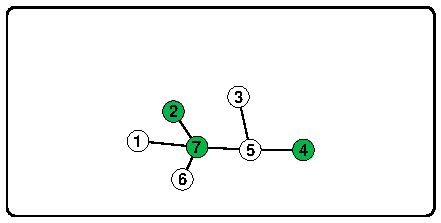
\includegraphics[clip,trim=0.1cm 0.1cm 0.1cm 0.1cm]{interaction_simulation1.pdf}};
    
    \node at (9,0) (2) {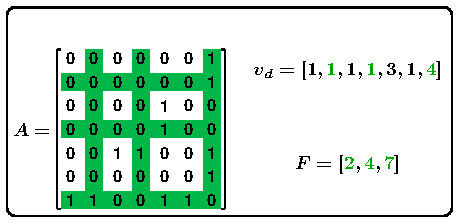
\includegraphics[clip,trim=0.1cm 0.1cm 0.1cm 0.1cm]{interaction_simulation2.pdf}};
    
    \node at (4.5,-5.3) (3) {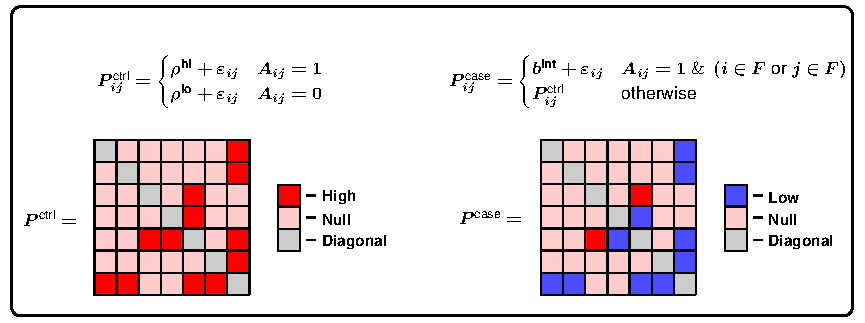
\includegraphics[clip,trim=0.1cm 0.1cm 0.1cm 0.1cm]{interaction_simulation3.pdf}};
    
    \node at (0,-10.08) (4) {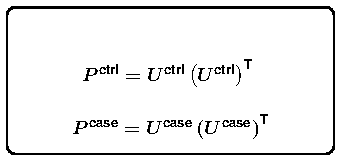
\includegraphics[clip,trim=0.1cm 0.1cm 0.1cm 0.1cm]{interaction_simulation4.pdf}};
    
    \node at (0,-14.22) (5) {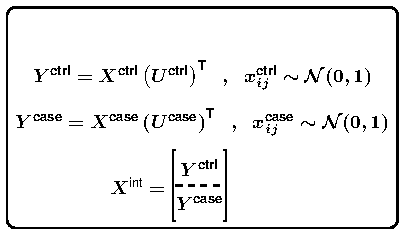
\includegraphics[clip,trim=0.1cm 0.1cm 0.1cm 0.1cm]{interaction_simulation5.pdf}};
    
    \node at (8.62,-10.82) (6) {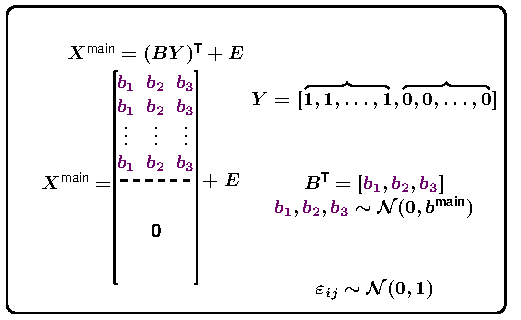
\includegraphics[clip,trim=0.1cm 0.1cm 0.1cm 0.1cm]{main_effect_added_to_interaction.pdf}};
    
    \node at (8.62,-15.17) (7) {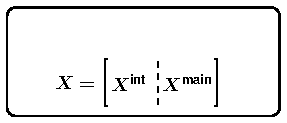
\includegraphics[clip,trim=0.1cm 0.1cm 0.1cm 0.1cm]{mixed_effects_combining_main-interaction.pdf}};
    
    %%%%%%%%%%%%%%%%%%%%%%%%%%%%%%%%%%%%%%% box 1 %%%%%%%%%%%%%%%%%%%%%%%%%%%%%%%%%%%%%%%%%%%%%%%
    \node[circle,draw,line width=0.2mm,xscale=1.4,yscale=1.4,fill=gray!40] at (-3.3,1.45) {};
    \node at (-3.3,1.45) {\textbf{1}};
    
    \node[xscale=1,yscale=1] at (0,0.9) {\textbf{Erd\H{o}s-R\'{e}nyi or Scale-free}};
    %\node[xscale=1,yscale=1] at (2.28,0.9) {\textbf{Erdos-Renyi}};
    %\node[xscale=1,yscale=1] at (0,0.9) {\textbf{or}};
    \node[xscale=1,yscale=1] at (0,1.45) {\textbf{Random graph}};
    %%%%%%%%%%%%%%%%%%%%%%%%%%%%%%%%%%%%%%% box 1 %%%%%%%%%%%%%%%%%%%%%%%%%%%%%%%%%%%%%%%%%%%%%%%
    
    %%%%%%%%%%%%%%%%%%%%%%%%%%%%%%%%%%%%%%% box 2 %%%%%%%%%%%%%%%%%%%%%%%%%%%%%%%%%%%%%%%%%%%%%%%
    \node[circle,draw,line width=0.2mm,xscale=1.4,yscale=1.4,fill=gray!40] at (5.55,1.45) {};
    \node at (5.55,1.45) {\textbf{2}};
    
    \node[xscale=1,yscale=1] at (7.5,1.45) {\textbf{Adjacency matrix}};
    \node[xscale=1,yscale=1] at (11,1.2) {\textbf{Degree vector}};
    \node[xscale=1,yscale=1] at (11,-0.4) {\textbf{Functional features}};
    %%%%%%%%%%%%%%%%%%%%%%%%%%%%%%%%%%%%%%% box 2 %%%%%%%%%%%%%%%%%%%%%%%%%%%%%%%%%%%%%%%%%%%%%%%
    
    %%%%%%%%%%%%%%%%%%%%%%%%%%%%%%%%%%%%%%% box 3 %%%%%%%%%%%%%%%%%%%%%%%%%%%%%%%%%%%%%%%%%%%%%%%
    \node[circle,draw,line width=0.2mm,xscale=1.4,yscale=1.4,fill=gray!40] at (-2.3,-3.01) {};
    \node at (-2.3,-3.01) {\textbf{3}};
    
    \node[xscale=1,yscale=1] at (4.5,-2.94) {\textbf{Correlation matrices}};
    
    \node[xscale=1,yscale=1] at (0.1,-4.7) {\textbf{Controls}};
    \node[xscale=1,yscale=1] at (7.65,-4.7) {\textbf{Cases}};
    %%%%%%%%%%%%%%%%%%%%%%%%%%%%%%%%%%%%%%% box 3 %%%%%%%%%%%%%%%%%%%%%%%%%%%%%%%%%%%%%%%%%%%%%%%
    
    %%%%%%%%%%%%%%%%%%%%%%%%%%%%%%%%%%%%%%% box 4 %%%%%%%%%%%%%%%%%%%%%%%%%%%%%%%%%%%%%%%%%%%%%%%
    \node[circle,draw,line width=0.2mm,xscale=1.4,yscale=1.4,fill=gray!40] at (-2.45,-9.17) {};
    \node at (-2.45,-9.17) {\textbf{4}};
    \node[xscale=1,yscale=1] at (0.2,-9.15) {\textbf{Cholesky decomposition}};
    %%%%%%%%%%%%%%%%%%%%%%%%%%%%%%%%%%%%%%% box 4 %%%%%%%%%%%%%%%%%%%%%%%%%%%%%%%%%%%%%%%%%%%%%%%
    
    %%%%%%%%%%%%%%%%%%%%%%%%%%%%%%%%%%%%%%% box 5 %%%%%%%%%%%%%%%%%%%%%%%%%%%%%%%%%%%%%%%%%%%%%%%
    \node[circle,draw,line width=0.2mm,xscale=1.4,yscale=1.4,fill=gray!40] at (-3,-12.67) {};
    \node at (-3,-12.67) {\textbf{5}};
    \node[xscale=1,yscale=1] at (0,-12.65) {\textbf{Interaction data}};
    %%%%%%%%%%%%%%%%%%%%%%%%%%%%%%%%%%%%%%% box 5 %%%%%%%%%%%%%%%%%%%%%%%%%%%%%%%%%%%%%%%%%%%%%%%
    
    %%%%%%%%%%%%%%%%%%%%%%%%%%%%%%%%%%%%%%% box 6 %%%%%%%%%%%%%%%%%%%%%%%%%%%%%%%%%%%%%%%%%%%%%%%
    \node[circle,draw,line width=0.2mm,xscale=1.4,yscale=1.4,fill=gray!40] at (4.65,-8.55) {};
    \node at (4.65,-8.55) {\textbf{6}};
    \node[xscale=1,yscale=1] at (6.85,-8.53) {\textbf{Design matrix}};
    
    \node[xscale=1,yscale=1] at (10.55,-8.85) {\textbf{Binary outcome}};
    
    \node[xscale=1,yscale=1] at (10.05,-9.3) {\textbf{Cases}};
    \node[xscale=1,yscale=1] at (11.74,-9.3) {\textbf{Controls}};
    
    \node[xscale=1,yscale=1] at (10.55,-10.7) {\textbf{Effect sizes}};
    
    \node[xscale=1,yscale=1] at (10.55,-12.55) {\textbf{Gaussian noise}};
    %%%%%%%%%%%%%%%%%%%%%%%%%%%%%%%%%%%%%%% box 6 %%%%%%%%%%%%%%%%%%%%%%%%%%%%%%%%%%%%%%%%%%%%%%%
    
    %%%%%%%%%%%%%%%%%%%%%%%%%%%%%%%%%%%%%%% box 7 %%%%%%%%%%%%%%%%%%%%%%%%%%%%%%%%%%%%%%%%%%%%%%%
    \node[circle,draw,line width=0.2mm,xscale=1.4,yscale=1.4,fill=gray!40] at (6.62,-14.57) {};
    \node at (6.62,-14.57) {\textbf{7}};
    \node[xscale=1,yscale=1] at (8.85,-14.55) {\textbf{Mixed effects data}};
    %%%%%%%%%%%%%%%%%%%%%%%%%%%%%%%%%%%%%%% box 7 %%%%%%%%%%%%%%%%%%%%%%%%%%%%%%%%%%%%%%%%%%%%%%%
    
\end{tikzpicture}
    
\end{document}